\documentclass[12pt]{scrreprt}
\usepackage{babel}
\usepackage{german}
\usepackage{times}
\usepackage{amssymb}
\usepackage{amsmath}
\usepackage{graphicx}
\usepackage{eurosym}
\usepackage{graphicx}

\subject{Diplomarbeit}
\title{Empfangsstation für globales Satellitenbodenstationsnetzwerk SatNOGS}
\author{Ritter Gabriel, Metzler Jakob}
\date{\today}
\publishers{Betreuer: Dipl.-Ing. König Christian}

\begin{document}
	
	\maketitle
	
	\chapter{Abstract}
	Ziel der Diplomarbeit ist es, eine funktionstüchtige Satelliten-Ground-Station aufzubauen, um mit 
	Satelliten im Amateurfunkband, vor allem auch dem CubeSat des STS1, kommunizieren zu können.\\
	
	
	Im ersten Schritt muss hierzu die Ground-Station selbst aufgebaut werden. Dazu gehören zum 
	Beispiel die Demodulation, Low-Noise-Amplification und ein Software-Defined-Radio. Sobald die 
	Ground-Station funktionstüchtig ist, sollen drei verschiedene Antennen-Typen gebaut und mit der 
	Ground-Station betrieben werden, um den besten Antennen-Typ für den Empfang der CubeSat-Daten zu ermitteln. Die empfangenen Daten sollen weiters über eine grafische Benutzeroberfläche 
	übersichtlich dargestellt werden können.\\
	
	
	Im letzten Schritt werden die verschiedenen Antennen charakterisiert und Werte wie die Richtcharakteristik und der Gain ermittelt.
	
	\chapter{Vorwort}
	Wir wollen allen danken die blabla so dankbar bla
	
	\tableofcontents
	\pagebreak
	
	\chapter{Theoretische Grundlagen}
	In diesem Kapitel werden die theoretischen Grundlagen der Antennen-und Leitertheorie gelegt sowie das SatNOGS Netzwerk näher erläutert.
	
	\section{SatNOGS-Netzwerk}
	Das SatNOGS-Netzwerk spielt eine zentrale Rolle in unserer Diplomarbeit und bietet hunderten Forschern, Amateurfunkern und Interessierten eine Plattform für verlässliche Kommunikation mit Satelliten.\\
	
	
	Das, was SatNOGS zu so einer attraktiven Lösung macht, ist der Fakt dass die Bodenstation um den ganzen Globus verteilt sind. Der große Vorteil davon ist, dass der Empfang von Satellitendaten nun über alle verfügbaren Empfangsstationen laufen kann.\\
	
	
	In Abbildung \ref{fig:Abb 3.1} wird die Topologie des SatNOGS-Netzwerkes abstrahiert dargestellt.
	Alle über das Netzwerk verfügbaren Bodenstationen sind mit SatNOGS-Servern verbunden. Auf diese Server kann über die Website bzw. API zugegriffen werden, welche die empfangenen Satellitendaten für alle Benutzer erreichbar macht.
	
	
	\begin{figure}[h]
		\begin{center}
			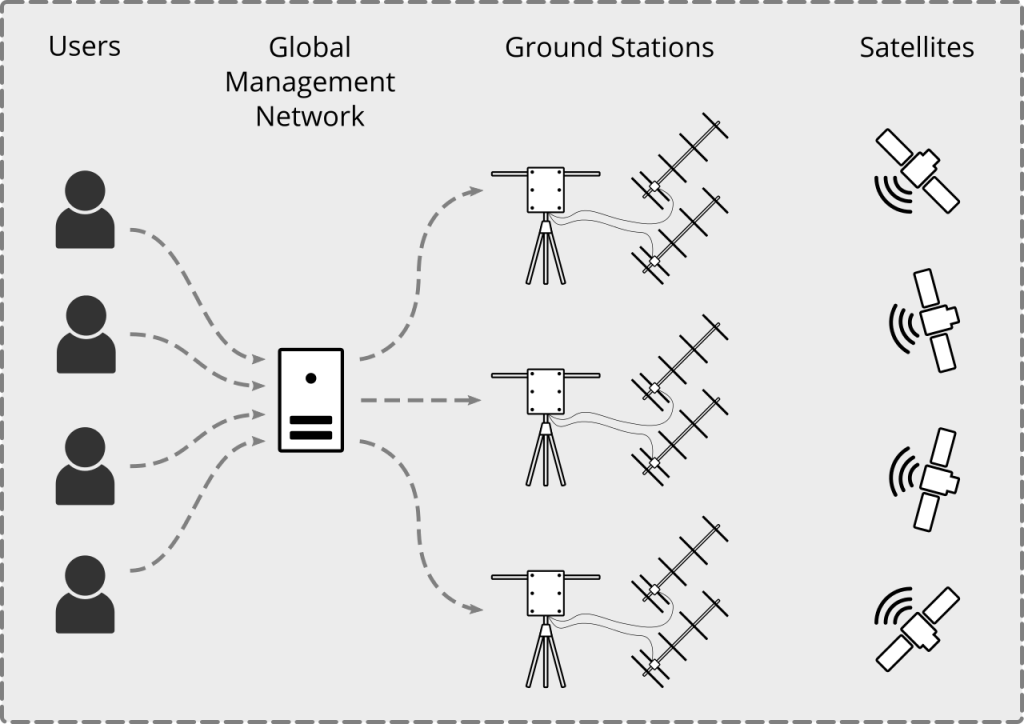
\includegraphics[width=10cm]{Doku - Grafiken/SatNOGS_explanation}
			\label{fig:Abb 3.1}
			\caption{SatNOGS-Netzwerk Erklärung}
		\end{center}
	\end{figure}
	
	Um näher auf den Ablauf des Datenempfangs und der benötigten Systemblöcke einzugehen wird auf Abbildung \ref{fig:Abb 3.2} verwiesen.\\	
	
	\begin{figure}[h]
		\begin{center}
			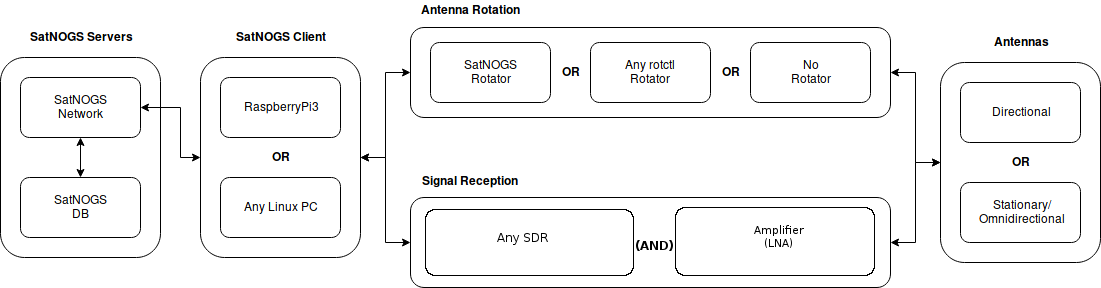
\includegraphics[width=16cm]{Doku - Grafiken/SatNOGS_BlockDiagram}
			\label{fig:Abb 3.2}
			\caption{SatNOGS-Systemtopologie}
		\end{center}
	\end{figure}

	Zum Empfang von Daten kommen zwei Antennentypen infrage: Direktionale oder omnidirektionale Antennen. Eine direktionale Antenne folgt dem Verlauf des Satelliten. Dies bringt den Vorteil mit sich, dass eine höhere Empfangsleistung erzielt, und somit klarere Daten empfangen werden, jedoch wird für solch ein Modell ein Rotator benötigt. Der Vorteil einer omnidirektionalen Antenne ist, dass kein teurer Rotator notwendig ist, allerdings können damit nur schwer brauchbare Daten empfangen werden.\\
	
	
	Für gerichtete Antennen können verschiedene Rotatoren benutzt werden, unter anderem der "SatNOGS-Rotator" sowie diverse Open-Source-Rotatoren und Rotatoren welche zum Verkauf stehen.\\
	
	
	Zur Demodulation der Daten sind ein SDR (Software Defined Radio) sowie ein LNA (Low Noise Amplifier) notwendig. Das SDR übernimmt softwaretechnisch Aufgaben welche normalerweise von Hardware übernommen werden (Demodulation, Filter, Mixer, etc...). Der LNA, wie der Name schon andeutet, ist für die Verstärkung kleiner Signale mit besonderer Rauscharmut verantwortlich. \\
	
	
	Die Aufgabe des SatNOGS Clients kann in der Regel von jedem Linux-PC oder RaspberryPi übernommen werden. Allerdings wird die Kompatibilität nur für den RaspberryPi3 und 4 garantiert.\\
	
	
	Der SatNOGS Client ist direkt mit den Servern verbunden
	\pagebreak
	
	\section{grundlegende Antennentheorie}
	\subsection{Einführung}
	
	\subsection{Antennenfeldzonen}
	
	\subsection{Polarisation}
	
	\subsection{Kenngrößen einer Antenne}
	
	\subsubsection{Antennengewinn}
	
	\subsubsection{Welligkeit}
	
	\subsubsection{Richtcharakteristik und Richtdiagramm}
	
	\subsubsection{Einfluss der Erde auf das Richtdiagramm}
	
	\subsection{Antennentypen}
	
	\subsubsection{Dipol}
		
	\subsubsection{QFH (Quadrifilar Helical Antenna)}
	

	
	\pagebreak
	
	\chapter{Hauptteil}
	\section{1. Antenne: Dipol}
	
	\section{2. Antenne: QFH (Quadrifilar Helical Antenna)}
	
	
	\pagebreak
	
	\chapter{Zusammenfassung}
	\pagebreak
	
	\chapter{Literaturverzeichnis}
	\pagebreak
	
	\chapter{Abkürzungsverzeichnis}
	\pagebreak
	
	\chapter{Begleitprotokoll}
	
	\chapter{Anhang}
	
	

	
\end{document}